\section{Implementation}
In the following we want to describe implementation specific details of both the simulator as well as the map editing application. We will elucidate problems we faced during the implementation and the integration of both applications and how we solved them. 
\subsection{Simulator}
Behind the user interface of the simulator a continuously running thread is mandated with updating the current state of the simulation with each tick, i.e. every 50ms. The thread execution is triggered by the globally governing SimulationController and its \textit{run}-method (fig.~\ref{fig:animthread}) appears refreshingly simple. Despite the apparent simplicity the design of the thread posed a range of problems. As is usual for Java UI frameworks, JavaFX also prohibits changes to UI objects by any thread other the main application thread, forcing us to submit each update that is to be escalated to the interface as a \textit{runnable} object to said application thread's execution queue. To reduce scheduling overhead we kept the AnimationThread's main loop as simple as possible, resulting in no more than four calls to the mentioned execution queue. 

\begin{figure}[h]
	\begin{center}
		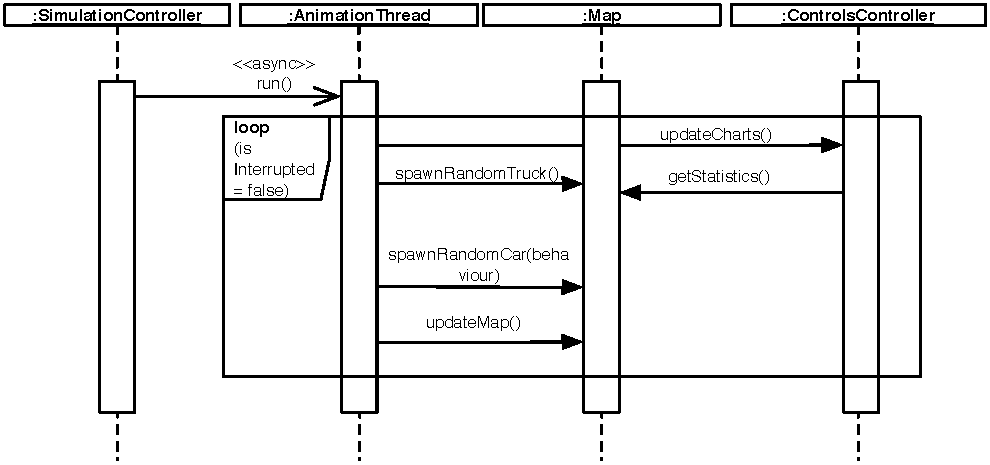
\includegraphics[width=\textwidth]{img/SD_animThread.pdf}
		\caption[Sequence Diagram of the Animation Thread]{Sequence Diagram of the Animation Thread}
		\label{fig:animthread}
	\end{center}
\end{figure}

With the multithreaded execution described above came concurrency related issues. The class Map contains a list to all vehicles currently present in the simulation. Whenever a vehicle is leaving the map, it notifies the SimulationController, which in turn removes the vehicle from the simulation. As the map's \textit{updateMap()} is constantly iterating through its list of vehicles, removing a vehicle from anywhere else than within this loop results in concurrency exceptions.

\begin{wrapfigure}{r}{0.45\textwidth}
	\begin{minipage}{0.45\textwidth}
		\begin{lstlisting}[caption={Car Removal}, label={lst:carRem}]
if(toBeRemoved.contains(v)){
	iter.remove();
	toBeRemoved.remove(v);
	continue;
}	
		\end{lstlisting}
	\end{minipage}
\end{wrapfigure}

In order to overcome this issue we considered both the traditional reader-writer-locking as well as the more advanced read-copy-update pattern, but eventually come to the conclusion but using either of them will introduce an additional scheduling (and implementation) overhead and hence only yield imperceptible performance improvements over the solution we employed (listing~\ref{lst:carRem}). As mentioned earlier, the \textit{updateMap()} method loops through all existing vehicles with each tick, we create a list of vehicles that are about to move the map within the next tick. As soon as the iterator (\textit{iter}) points to a vehicle \textit{v} that is on the \textit{toBeRemoved} list, it is removed and the loop skips one iteration.  

In order to ease the communication between model classes and the \textit{SimulationController} as well as the application classes \textit{MainApp} and \textit{EditorApp} we faced a design decision between the traditional observer pattern and the singleton pattern that allows static access to the required instances. We decided in favour of the singleton pattern, because the situations in which the model communicates with the \textit{SimulationController} are manifold and access to the singleton instance allows for fairly simple communication flows.

\subsection{Testing}
In order to meet all the requirements specified at the beginning of the project, testing forms an integral part in this process. Within the Agile development framework, we felt that Feature Driven Development (FDD) is most adaptable process suited for this project. Hence we decided to test the codes iteratively at the end of each development cycle. We foresaw that writing testing code in a concurrent fashion with the development team may not be an effective way, given the fact that the testing codes may not be working for the final product as incremental changes were made throughout the development. Therefore peer reviewing were conducted at early stage to ensure  code quality is kept to standard, that is, each method should be written explicitly to address the problem that needs to be solved. In such manner, we can be assured of a rigid foundation (i.e. the software model) before we even attempt to adding more complicated features.

As the software becomes mature, unit testings were added to the project. We conducted unit testings in JUnit with the support of JemmyFX and ScenicView. JemmyFX is a third party library for testing JavaFX application. It is a test harness which allows the user to simulate user input, i.e. click buttons, entering data. In particular, JemmyFX defines how to get a list of scenes, nodes items, and get text of a \textit{javafx.scene.control.Label} (listing~\ref{lst:checkBox}). We have mainly used this for UI testing. 


\begin{minipage}{0.9\textwidth}
	\begin{lstlisting}[caption={Use JemmyFX syntax to find a checkBox element}, label={lst:checkBox}]

//Identifying the input checkBox element exist
assertEquals(CheckBox.class, new LabeledDock(scene.asParent(), checkBoxName, StringComparePolicy.EXACT).wrap().getControl().getClass());

//Find the label of the checkBox 
LabeledDock cb = new LabeledDock(scene.asParent(), checkBoxName, StringComparePolicy.EXACT);

	\end{lstlisting}
\end{minipage}

Using ScenicView helped us to understand what the UI was built from, allowing us and any other future developers to quickly and efficiently query the properties of a particular element, i.e. finding the properties of a JavaFX button (fig.~\ref{fig:scenicview}). ScenicView provide tree structure and highlight the item upon it is selected. In the case of unable identify an elements within the source code, this has been particularly helpful.  
\begin{figure}[h]
	\begin{center}
		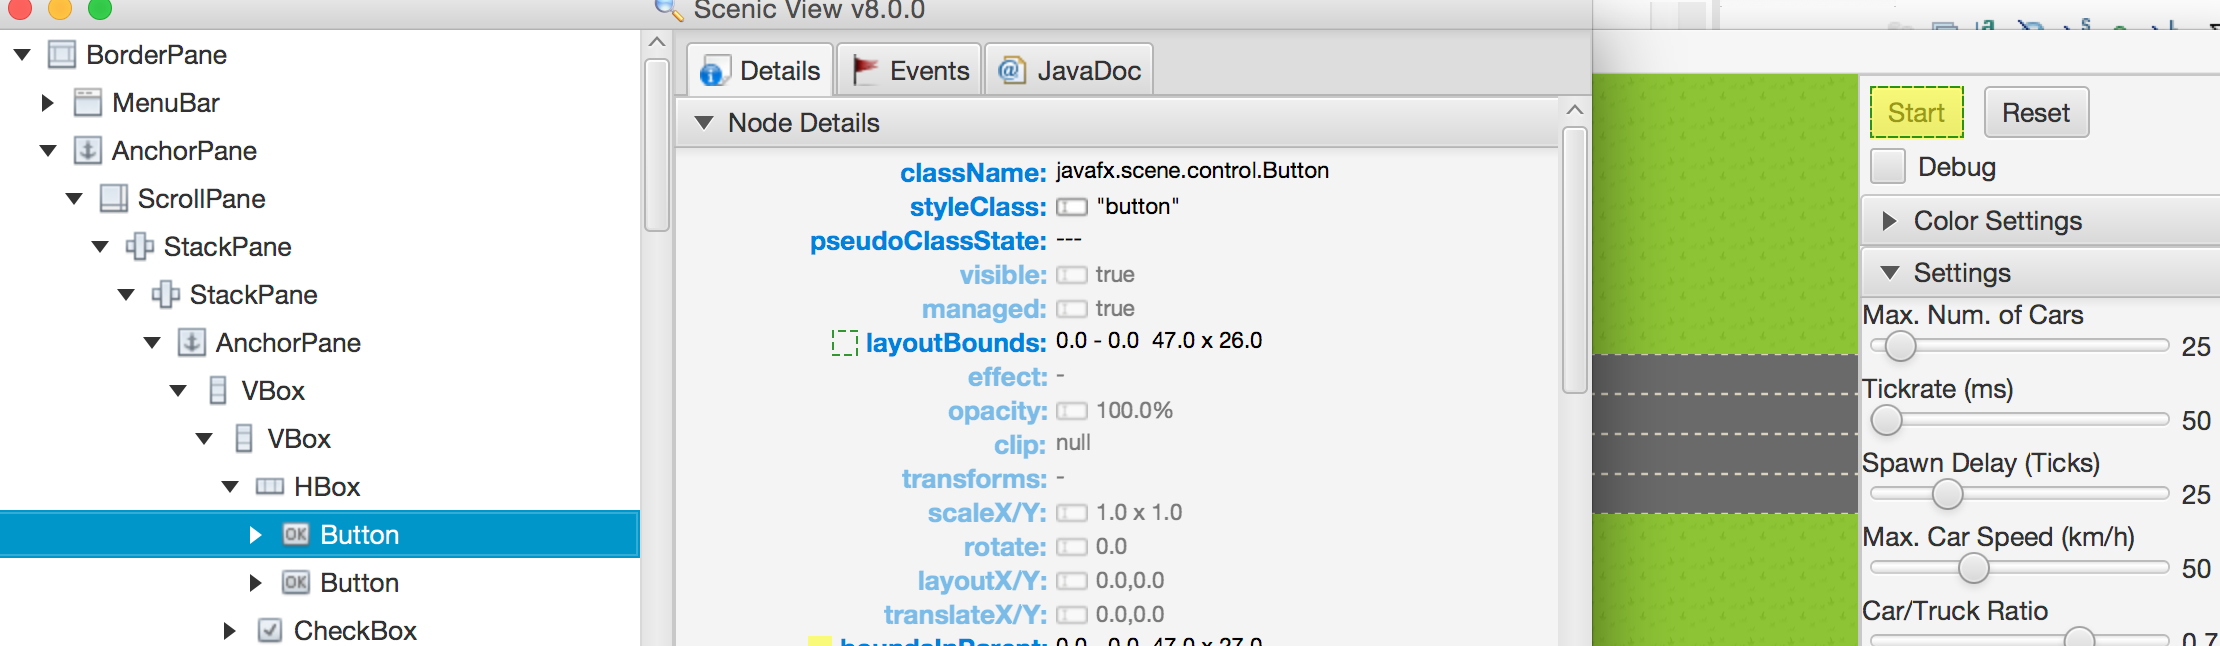
\includegraphics[width=\textwidth]{img/scenicView.png}
		\caption[Identifying properties of Start button with ScenicView]{Identifying properties of Start button with ScenicView}
		\label{fig:scenicview}
	\end{center}
\end{figure}

